\documentclass[11pt,a4paper]{ctexart}
\usepackage[utf8]{inputenc}
\usepackage{amsmath}
\usepackage{graphicx}
\usepackage{booktabs}
\usepackage{longtable}
\usepackage{geometry}
\usepackage{hyperref}
\usepackage{float}
\usepackage{amssymb}
\usepackage{xcolor}

\geometry{left=2.5cm,right=2.5cm,top=3cm,bottom=3cm}
\hypersetup{colorlinks=true, linkcolor=blue, citecolor=blue, urlcolor=blue}

% Helper: red text for out-of-range voltage
\newcommand{\vred}[1]{\textcolor{red}{\textbf{#1}}}

\title{低频交流输电系统 (LFAC) 10 节点潮流计算\\CloudPSS 仿真平台线路参数双模式对比报告}
\author{新能源工作室}
\date{\today}

\begin{document}

\maketitle

\section{系统说明}
本报告使用 \textbf{CloudPSS 仿真平台线路参数} 进行 10 节点低频交流海上风电送出系统的潮流计算。与原 case 的主要区别在于线路部分的 R/X/B 参数和汇集线路长度采用 CloudPSS 平台参数（统一 10km），变压器阻抗（主变+箱变）仍然保留。

节点电压安全范围：$0.97 \sim 1.07$ pu。表中超出该范围的电压值以 \vred{红色} 标注。

\begin{table}[H]
\centering
\caption{CloudPSS 线路参数}
\begin{tabular}{lccc}
\toprule
参数 & 汇集线路 (1-8$\to$9) & 送出线路 (9$\to$10) & 单位 \\
\midrule
长度 & 10 (统一) & 265 & km \\
频率 & 20 & 20 & Hz \\
正序电阻 & 0.01158 & 0.01158 & $\Omega$/km \\
正序感抗 & 0.02991 & 0.02991 & $\Omega$/km \\
正序容抗 & 0.3316 & 0.3316 & M$\Omega\cdot$km \\
\midrule
\multicolumn{4}{l}{变压器阻抗：主变 $U_k\%=14\%$，箱变 $U_k\%=7.5\%$（与原 case 一致）} \\
\bottomrule
\end{tabular}
\end{table}

\begin{table}[H]
\centering
\caption{10 节点系统定义}
\begin{tabular}{llll}
\toprule
节点编号 & 类型 & 额定电压 (kV) & 说明 \\
\midrule
1 -- 8 & PQ & 37 & 风电场 (WF1 -- WF8) \\
9 & PQ & 230 & 汇集站 (Collection Bus) \\
10 & Slack & 230 & 变频变流器站/平衡节点 (M3C + Grid) \\
\bottomrule
\end{tabular}
\end{table}

%% ========================= Part I =============================
\section{Part I: Constant Q Mode (Q=0)}
在该模式下，所有风电机组（节点 1--8）的无功出力固定为 0，系统完全依靠变频站和平衡节点支撑电压。

\subsection{Part I.1 潮流计算收敛性}
\begin{table}[H]
\centering
\caption{Constant Q 模式收敛性}
\begin{tabular}{lcc}
\toprule
场景 & Python 收敛 & 结论 \\
\midrule
标准工况 & \checkmark & 正常 \\
轻载工况 & \checkmark & 正常 \\
重载工况 & \checkmark & 正常 \\
故障工况 & \checkmark & 正常 \\
\bottomrule
\end{tabular}
\end{table}

\subsection{Part I.2 P-V 灵敏度扫描 (10\% -- 150\%)}
\begin{figure}[H]
\centering

\includegraphics[width=0.85\textwidth]{pf_figs/pv_sweep_q_const.png}
\caption{Constant Q 模式各节点 P-V 曲线 (CloudPSS 线路参数)}
\end{figure}

\subsection{Part I.3 详细潮流结果}

% ---- Q=0 Standard ----
\subsubsection{标准工况 潮流详表}
\begin{longtable}{cccccc}
\caption{Constant Q -- 标准工况} \\
\toprule
节点 & 类型 & Vm (pu) & Va (deg) & P Gen (MW) & Q Gen (Mvar) \\
\midrule
\endhead
1 & 1 & 0.9954 & 21.39 & 200.0 & 0.0 \\
2 & 1 & 0.9962 & 21.35 & 100.0 & 0.0 \\
3 & 1 & 0.9954 & 21.39 & 200.0 & 0.0 \\
4 & 1 & 0.9962 & 21.35 & 100.0 & 0.0 \\
5 & 1 & 0.9962 & 21.35 & 100.0 & 0.0 \\
6 & 1 & 0.9962 & 21.35 & 100.0 & 0.0 \\
7 & 1 & 0.9962 & 21.35 & 100.0 & 0.0 \\
8 & 1 & 0.9962 & 21.35 & 100.0 & 0.0 \\
9 & 1 & 1.0176 & 9.07 & 0.0 & 0.0 \\
10 & 3 & 1.0000 & 0.00 & $-$941.8 & 311.1 \\
\bottomrule
\end{longtable}

\begin{figure}[H]
\centering

\includegraphics[width=0.7\textwidth]{pf_figs/res_q_const_standard.png}
\caption{Constant Q 标准工况剖面}
\end{figure}

% ---- Q=0 Low ----
\subsubsection{轻载工况 潮流详表}
\begin{longtable}{cccccc}
\caption{Constant Q -- 轻载工况} \\
\toprule
节点 & 类型 & Vm (pu) & Va (deg) & P Gen (MW) & Q Gen (Mvar) \\
\midrule
\endhead
1 & 1 & 1.0113 & 9.09 & 60.0 & 0.0 \\
2 & 1 & 1.0129 & 9.07 & 30.0 & 0.0 \\
3 & 1 & 1.0113 & 9.09 & 60.0 & 0.0 \\
4 & 1 & 1.0129 & 9.07 & 30.0 & 0.0 \\
5 & 1 & 1.0129 & 9.07 & 30.0 & 0.0 \\
6 & 1 & 1.0129 & 9.07 & 30.0 & 0.0 \\
7 & 1 & 1.0129 & 9.07 & 30.0 & 0.0 \\
8 & 1 & 1.0129 & 9.07 & 30.0 & 0.0 \\
9 & 1 & 1.0162 & 2.53 & 0.0 & 0.0 \\
10 & 3 & 1.0000 & 0.00 & $-$294.9 & $-$8.7 \\
\bottomrule
\end{longtable}

\begin{figure}[H]
\centering

\includegraphics[width=0.7\textwidth]{pf_figs/res_q_const_low.png}
\caption{Constant Q 轻载工况剖面}
\end{figure}

% ---- Q=0 Heavy ----
\subsubsection{重载工况 潮流详表}
\begin{longtable}{cccccc}
\caption{Constant Q -- 重载工况} \\
\toprule
节点 & 类型 & Vm (pu) & Va (deg) & P Gen (MW) & Q Gen (Mvar) \\
\midrule
\endhead
1 & 1 & 0.9885 & 23.37 & 220.0 & 0.0 \\
2 & 1 & 0.9893 & 23.32 & 110.0 & 0.0 \\
3 & 1 & 0.9885 & 23.37 & 220.0 & 0.0 \\
4 & 1 & 0.9893 & 23.32 & 110.0 & 0.0 \\
5 & 1 & 0.9893 & 23.32 & 110.0 & 0.0 \\
6 & 1 & 0.9893 & 23.32 & 110.0 & 0.0 \\
7 & 1 & 0.9893 & 23.32 & 110.0 & 0.0 \\
8 & 1 & 0.9893 & 23.32 & 110.0 & 0.0 \\
9 & 1 & 1.0143 & 10.09 & 0.0 & 0.0 \\
10 & 3 & 1.0000 & 0.00 & $-$1028.6 & 386.2 \\
\bottomrule
\end{longtable}

\begin{figure}[H]
\centering

\includegraphics[width=0.7\textwidth]{pf_figs/res_q_const_heavy.png}
\caption{Constant Q 重载工况剖面}
\end{figure}

% ---- Q=0 Trip ----
\subsubsection{故障工况 潮流详表}
\begin{longtable}{cccccc}
\caption{Constant Q -- 故障工况} \\
\toprule
节点 & 类型 & Vm (pu) & Va (deg) & P Gen (MW) & Q Gen (Mvar) \\
\midrule
\endhead
1 & 4 & 1.0000 & 0.00 & 0.0 & 0.0 \\
2 & 1 & 0.9955 & 19.53 & 100.0 & 0.0 \\
3 & 1 & 0.9947 & 19.57 & 200.0 & 0.0 \\
4 & 1 & 0.9955 & 19.53 & 100.0 & 0.0 \\
5 & 1 & 0.9955 & 19.53 & 100.0 & 0.0 \\
6 & 1 & 0.9955 & 19.53 & 100.0 & 0.0 \\
7 & 1 & 0.9955 & 19.53 & 100.0 & 0.0 \\
8 & 1 & 0.9955 & 19.53 & 100.0 & 0.0 \\
9 & 1 & 1.0169 & 7.23 & 0.0 & 0.0 \\
10 & 3 & 1.0000 & 0.00 & $-$762.8 & 215.5 \\
\bottomrule
\end{longtable}

\begin{figure}[H]
\centering

\includegraphics[width=0.7\textwidth]{pf_figs/res_q_const_trip.png}
\caption{Constant Q 故障工况剖面}
\end{figure}

%% ========================= Part II =============================
\section{Part II: Constant PF Mode (PF=0.98)}
在该模式下，风电机组按 0.98 滞后功率因数运行，无功出力随有功同步变化，提供就地电压支撑。

\subsection{Part II.1 潮流计算收敛性}
\begin{table}[H]
\centering
\caption{Constant PF 模式收敛性}
\begin{tabular}{lcc}
\toprule
场景 & Python 收敛 & 结论 \\
\midrule
标准工况 & \checkmark & 正常 \\
轻载工况 & \checkmark & 正常 \\
重载工况 & \checkmark & 正常 \\
故障工况 & \checkmark & 正常 \\
\bottomrule
\end{tabular}
\end{table}

\subsection{Part II.2 P-V 灵敏度扫描 (10\% -- 150\%)}
\begin{figure}[H]
\centering

\includegraphics[width=0.85\textwidth]{pf_figs/pv_sweep_pf_const.png}
\caption{Constant PF 模式各节点 P-V 曲线 (CloudPSS 线路参数)}
\end{figure}

\subsection{Part II.3 详细潮流结果}

% ---- PF Standard ----
\subsubsection{标准工况 潮流详表}
\begin{longtable}{cccccc}
\caption{Constant PF -- 标准工况} \\
\toprule
节点 & 类型 & Vm (pu) & Va (deg) & P Gen (MW) & Q Gen (Mvar) \\
\midrule
\endhead
1 & 1 & \vred{1.0746} & 19.06 & 200.0 & 40.6 \\
2 & 1 & \vred{1.0753} & 19.03 & 100.0 & 20.3 \\
3 & 1 & \vred{1.0746} & 19.06 & 200.0 & 40.6 \\
4 & 1 & \vred{1.0753} & 19.03 & 100.0 & 20.3 \\
5 & 1 & \vred{1.0753} & 19.03 & 100.0 & 20.3 \\
6 & 1 & \vred{1.0753} & 19.03 & 100.0 & 20.3 \\
7 & 1 & \vred{1.0753} & 19.03 & 100.0 & 20.3 \\
8 & 1 & \vred{1.0753} & 19.03 & 100.0 & 20.3 \\
9 & 1 & 1.0518 & 8.04 & 0.0 & 0.0 \\
10 & 3 & 1.0000 & 0.00 & $-$947.2 & 68.6 \\
\bottomrule
\end{longtable}

\begin{figure}[H]
\centering

\includegraphics[width=0.7\textwidth]{pf_figs/res_pf_const_standard.png}
\caption{Constant PF 标准工况剖面}
\end{figure}

% ---- PF Low ----
\subsubsection{轻载工况 潮流详表}
\begin{longtable}{cccccc}
\caption{Constant PF -- 轻载工况} \\
\toprule
节点 & 类型 & Vm (pu) & Va (deg) & P Gen (MW) & Q Gen (Mvar) \\
\midrule
\endhead
1 & 1 & 1.0438 & 8.60 & 60.0 & 12.2 \\
2 & 1 & 1.0453 & 8.58 & 30.0 & 6.1 \\
3 & 1 & 1.0438 & 8.60 & 60.0 & 12.2 \\
4 & 1 & 1.0453 & 8.58 & 30.0 & 6.1 \\
5 & 1 & 1.0453 & 8.58 & 30.0 & 6.1 \\
6 & 1 & 1.0453 & 8.58 & 30.0 & 6.1 \\
7 & 1 & 1.0453 & 8.58 & 30.0 & 6.1 \\
8 & 1 & 1.0453 & 8.58 & 30.0 & 6.1 \\
9 & 1 & 1.0254 & 2.31 & 0.0 & 0.0 \\
10 & 3 & 1.0000 & 0.00 & $-$294.8 & $-$70.7 \\
\bottomrule
\end{longtable}

\begin{figure}[H]
\centering

\includegraphics[width=0.7\textwidth]{pf_figs/res_pf_const_low.png}
\caption{Constant PF 轻载工况剖面}
\end{figure}

% ---- PF Heavy ----
\subsubsection{重载工况 潮流详表}
\begin{longtable}{cccccc}
\caption{Constant PF -- 重载工况} \\
\toprule
节点 & 类型 & Vm (pu) & Va (deg) & P Gen (MW) & Q Gen (Mvar) \\
\midrule
\endhead
1 & 1 & \vred{1.0762} & 20.61 & 220.0 & 44.7 \\
2 & 1 & \vred{1.0768} & 20.57 & 110.0 & 22.3 \\
3 & 1 & \vred{1.0762} & 20.61 & 220.0 & 44.7 \\
4 & 1 & \vred{1.0768} & 20.57 & 110.0 & 22.3 \\
5 & 1 & \vred{1.0768} & 20.57 & 110.0 & 22.3 \\
6 & 1 & \vred{1.0768} & 20.57 & 110.0 & 22.3 \\
7 & 1 & \vred{1.0768} & 20.57 & 110.0 & 22.3 \\
8 & 1 & \vred{1.0768} & 20.57 & 110.0 & 22.3 \\
9 & 1 & 1.0533 & 8.89 & 0.0 & 0.0 \\
10 & 3 & 1.0000 & 0.00 & $-$1036.4 & 108.8 \\
\bottomrule
\end{longtable}

\begin{figure}[H]
\centering

\includegraphics[width=0.7\textwidth]{pf_figs/res_pf_const_heavy.png}
\caption{Constant PF 重载工况剖面}
\end{figure}

% ---- PF Trip ----
\subsubsection{故障工况 潮流详表}
\begin{longtable}{cccccc}
\caption{Constant PF -- 故障工况} \\
\toprule
节点 & 类型 & Vm (pu) & Va (deg) & P Gen (MW) & Q Gen (Mvar) \\
\midrule
\endhead
1 & 4 & 1.0000 & 0.00 & 0.0 & 0.0 \\
2 & 1 & 1.0671 & 17.62 & 100.0 & 20.3 \\
3 & 1 & 1.0664 & 17.66 & 200.0 & 40.6 \\
4 & 1 & 1.0671 & 17.62 & 100.0 & 20.3 \\
5 & 1 & 1.0671 & 17.62 & 100.0 & 20.3 \\
6 & 1 & 1.0671 & 17.62 & 100.0 & 20.3 \\
7 & 1 & 1.0671 & 17.62 & 100.0 & 20.3 \\
8 & 1 & 1.0671 & 17.62 & 100.0 & 20.3 \\
9 & 1 & 1.0438 & 6.47 & 0.0 & 0.0 \\
10 & 3 & 1.0000 & 0.00 & $-$765.7 & 27.5 \\
\bottomrule
\end{longtable}

\begin{figure}[H]
\centering

\includegraphics[width=0.7\textwidth]{pf_figs/res_pf_const_trip.png}
\caption{Constant PF 故障工况剖面}
\end{figure}

%% ========================= Part III =============================
\section{Part III: Constant PF Mode (PF=0.99)}
在该模式下，风电机组按 0.99 滞后功率因数运行。相比 0.98 模式，其无功出力减小，旨在抑制重载下的电压过越（>1.07 pu）。

\subsection{Part III.1 潮流计算收敛性}
\begin{table}[H]
\centering
\caption{Constant PF (0.99) 模式收敛性}
\begin{tabular}{lcc}
\toprule
场景 & Python 收敛 & 结论 \\
\midrule
标准工况 & \checkmark & 正常 \\
轻载工况 & \checkmark & 正常 \\
重载工况 & \checkmark & 正常 \\
故障工况 & \checkmark & 正常 \\
\bottomrule
\end{tabular}
\end{table}

\subsection{Part III.2 P-V 灵敏度扫描 (10\% -- 150\%)}
\begin{figure}[H]
\centering
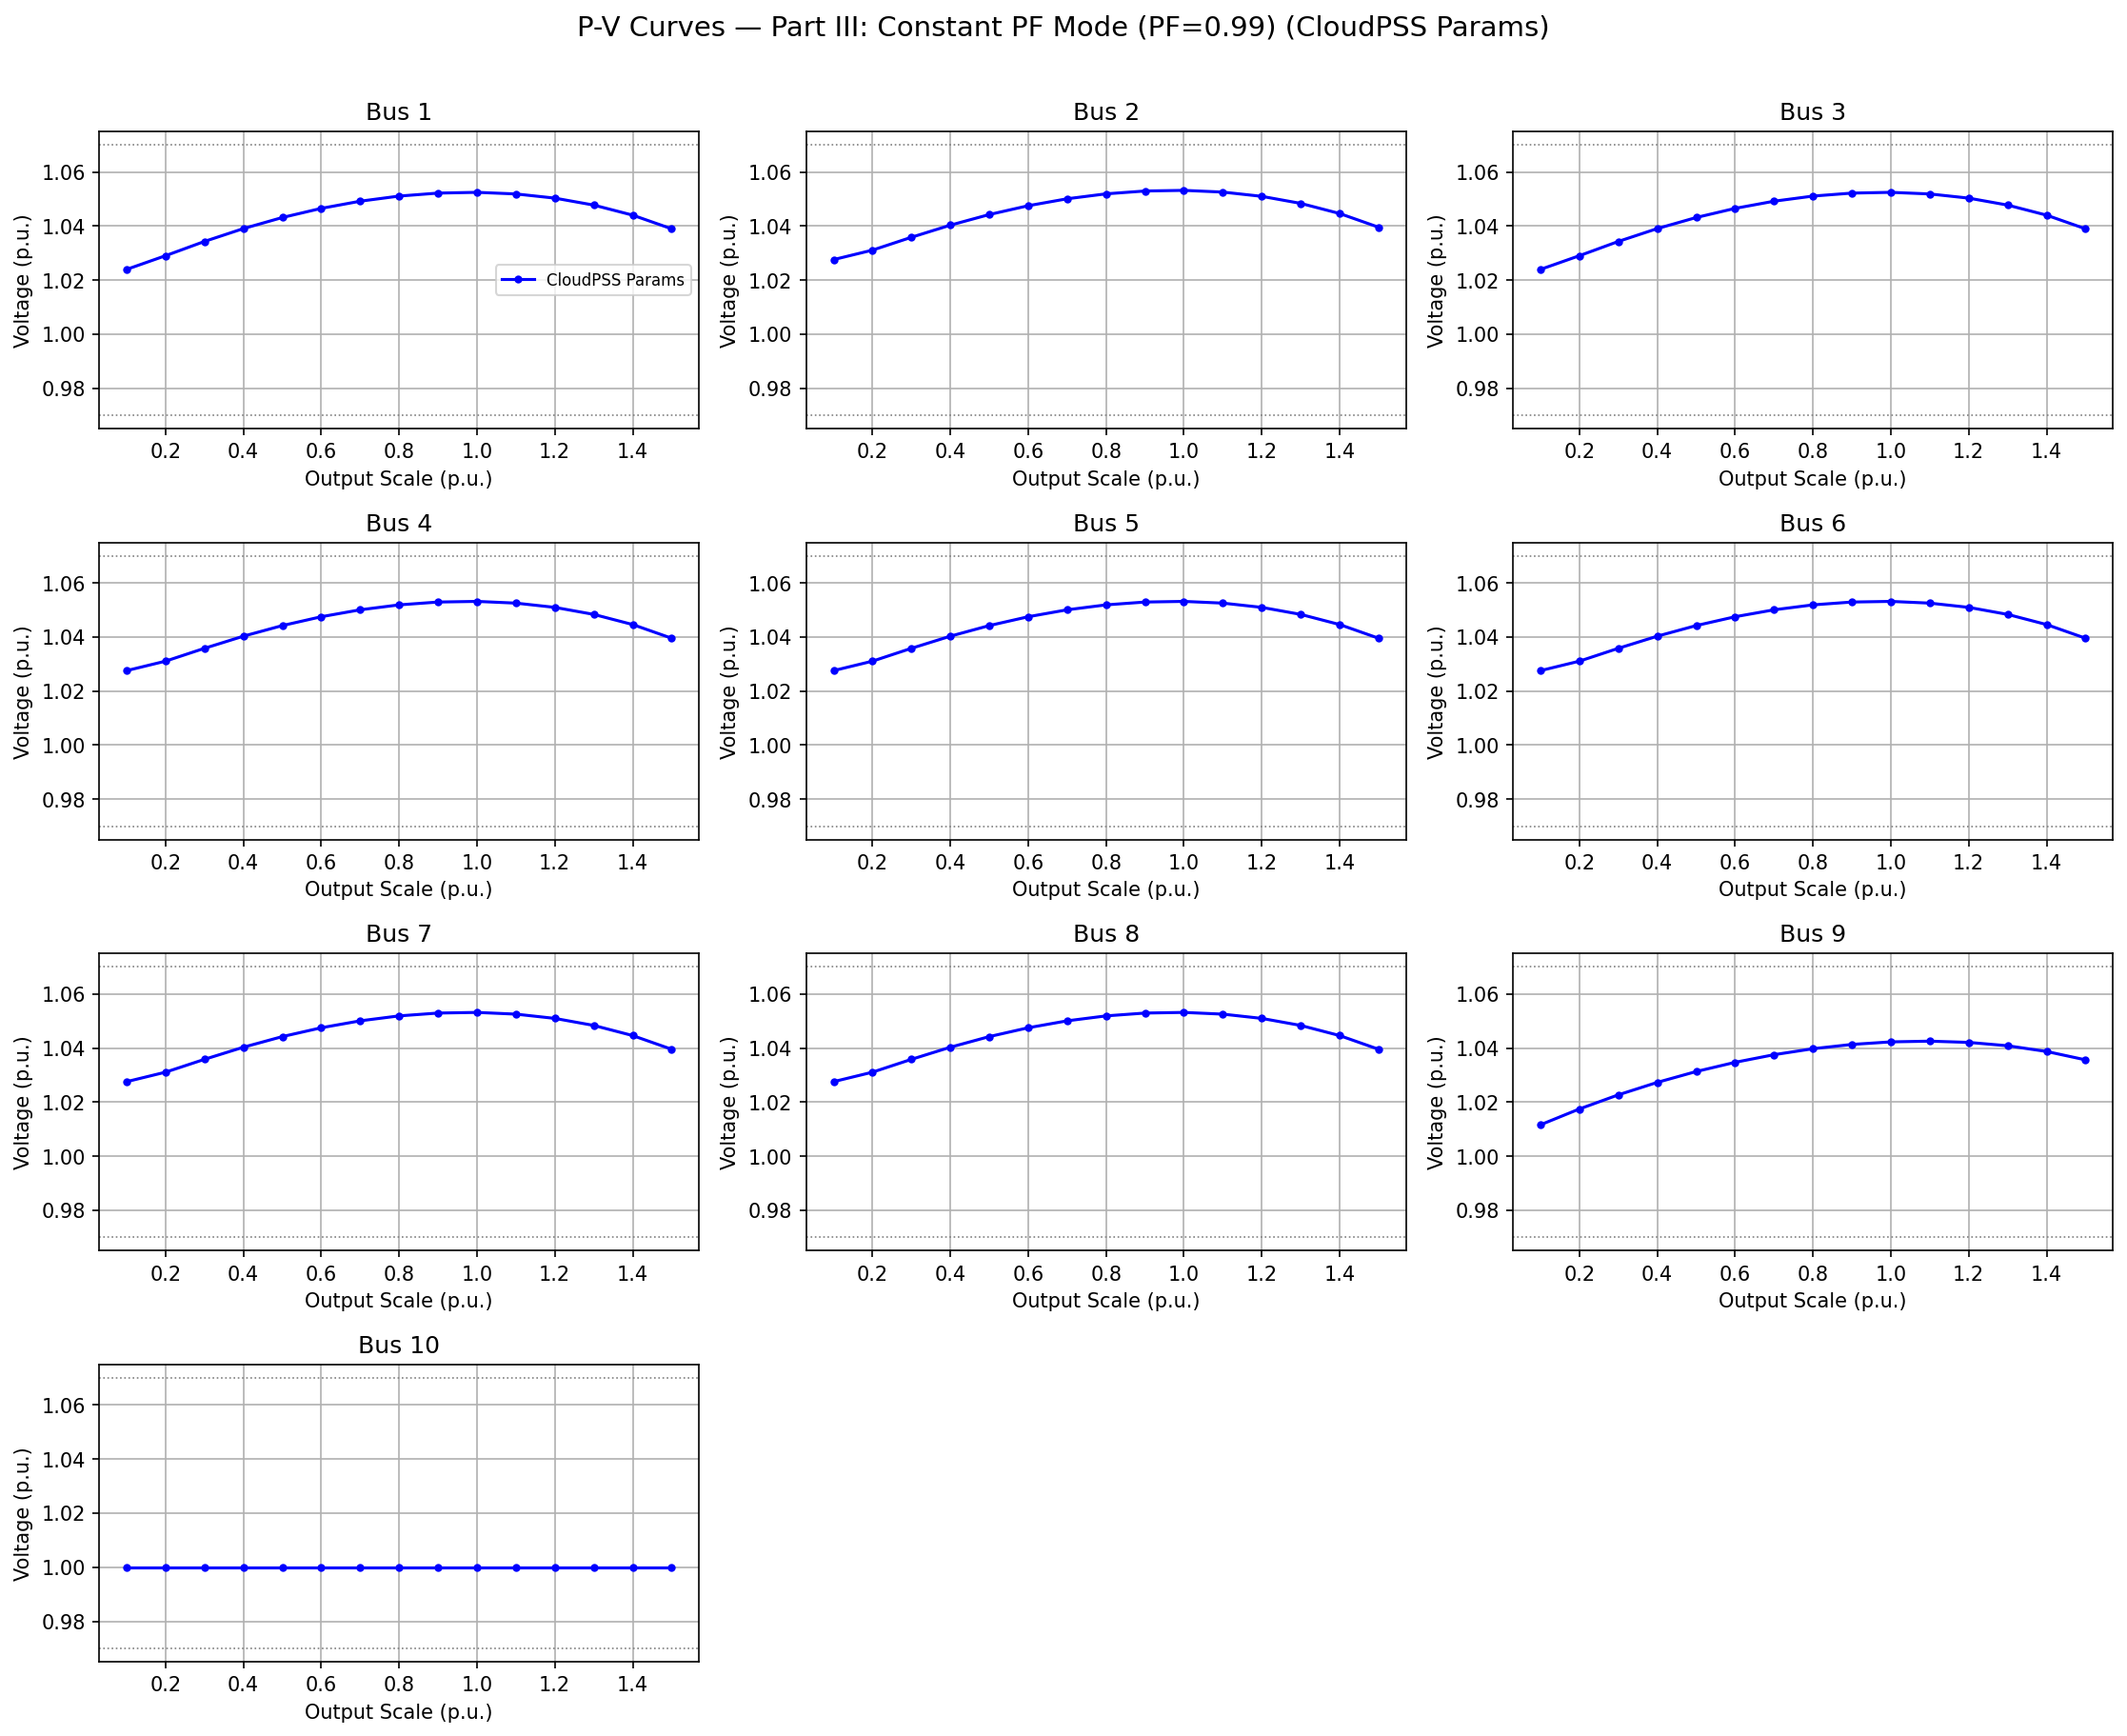
\includegraphics[width=0.85\textwidth]{pf_figs/pv_sweep_pf_099.png}
\caption{Constant PF (0.99) 模式各节点 P-V 曲线 (CloudPSS 线路参数)}
\end{figure}

\subsection{Part III.3 详细潮流结果}

\subsubsection{标准工况 潮流详表}
\begin{longtable}{cccccc}
\caption{Constant PF (0.99) -- 标准工况} \\
\toprule
节点 & 类型 & Vm (pu) & Va (deg) & P Gen (MW) & Q Gen (Mvar) \\
\midrule
\endhead
1 & 1 & 1.0525 & 19.69 & 200.0 & 28.5 \\
2 & 1 & 1.0532 & 19.65 & 100.0 & 14.2 \\
3 & 1 & 1.0525 & 19.69 & 200.0 & 28.5 \\
4 & 1 & 1.0532 & 19.65 & 100.0 & 14.2 \\
5 & 1 & 1.0532 & 19.65 & 100.0 & 14.2 \\
6 & 1 & 1.0532 & 19.65 & 100.0 & 14.2 \\
7 & 1 & 1.0532 & 19.65 & 100.0 & 14.2 \\
8 & 1 & 1.0532 & 19.65 & 100.0 & 14.2 \\
9 & 1 & 1.0423 & 8.33 & 0.0 & 0.0 \\
10 & 3 & 1.0000 & 0.00 & $-$946.3 & 136.3 \\
\bottomrule
\end{longtable}

\begin{figure}[H]
\centering
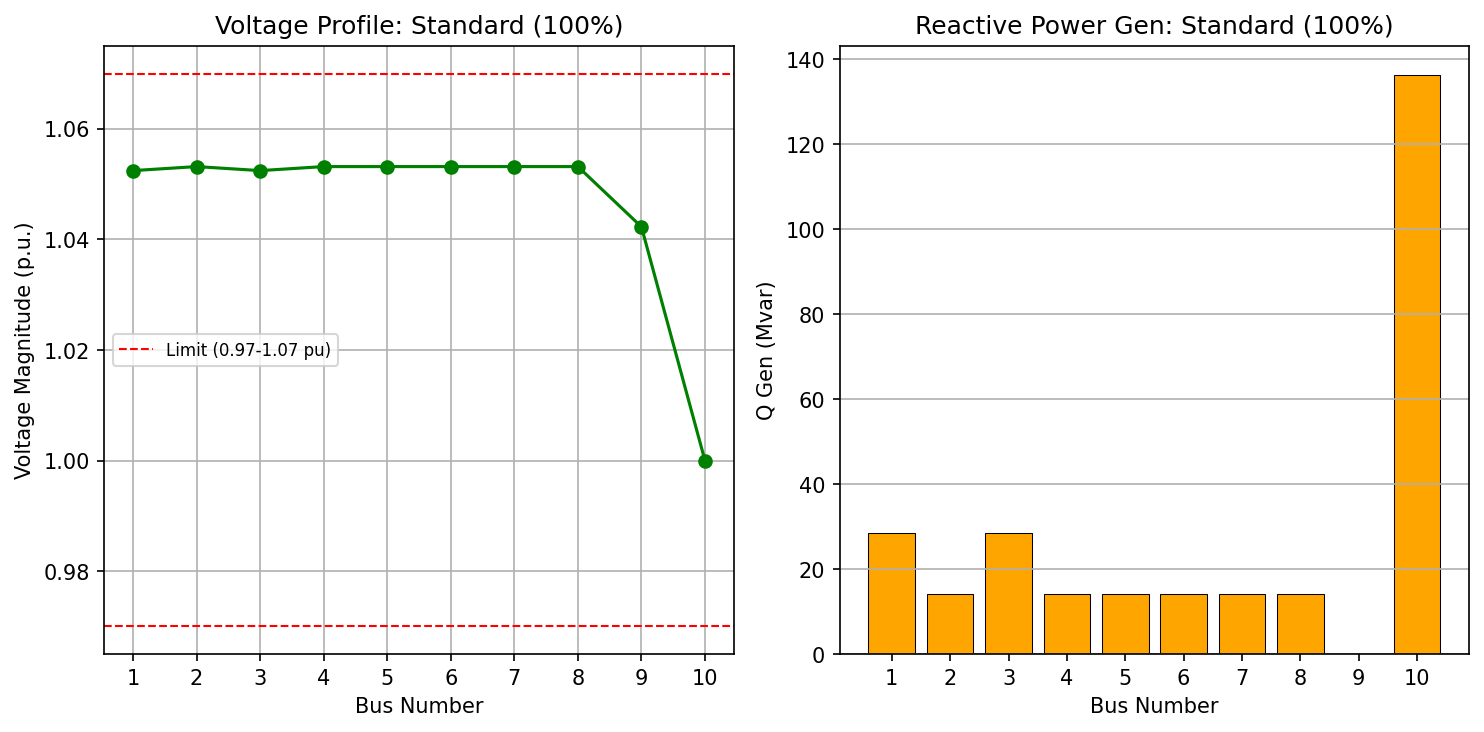
\includegraphics[width=0.7\textwidth]{pf_figs/res_pf_099_standard.png}
\caption{Constant PF (0.99) 标准工况剖面}
\end{figure}

\subsubsection{轻载工况 潮流详表}
\begin{longtable}{cccccc}
\caption{Constant PF (0.99) -- 轻载工况} \\
\toprule
节点 & 类型 & Vm (pu) & Va (deg) & P Gen (MW) & Q Gen (Mvar) \\
\midrule
\endhead
1 & 1 & 1.0343 & 8.74 & 60.0 & 8.5 \\
2 & 1 & 1.0358 & 8.72 & 30.0 & 4.3 \\
3 & 1 & 1.0343 & 8.74 & 60.0 & 8.5 \\
4 & 1 & 1.0358 & 8.72 & 30.0 & 4.3 \\
5 & 1 & 1.0358 & 8.72 & 30.0 & 4.3 \\
6 & 1 & 1.0358 & 8.72 & 30.0 & 4.3 \\
7 & 1 & 1.0358 & 8.72 & 30.0 & 4.3 \\
8 & 1 & 1.0358 & 8.72 & 30.0 & 4.3 \\
9 & 1 & 1.0227 & 2.37 & 0.0 & 0.0 \\
10 & 3 & 1.0000 & 0.00 & $-$294.9 & $-$32.5 \\
\bottomrule
\end{longtable}

\begin{figure}[H]
\centering
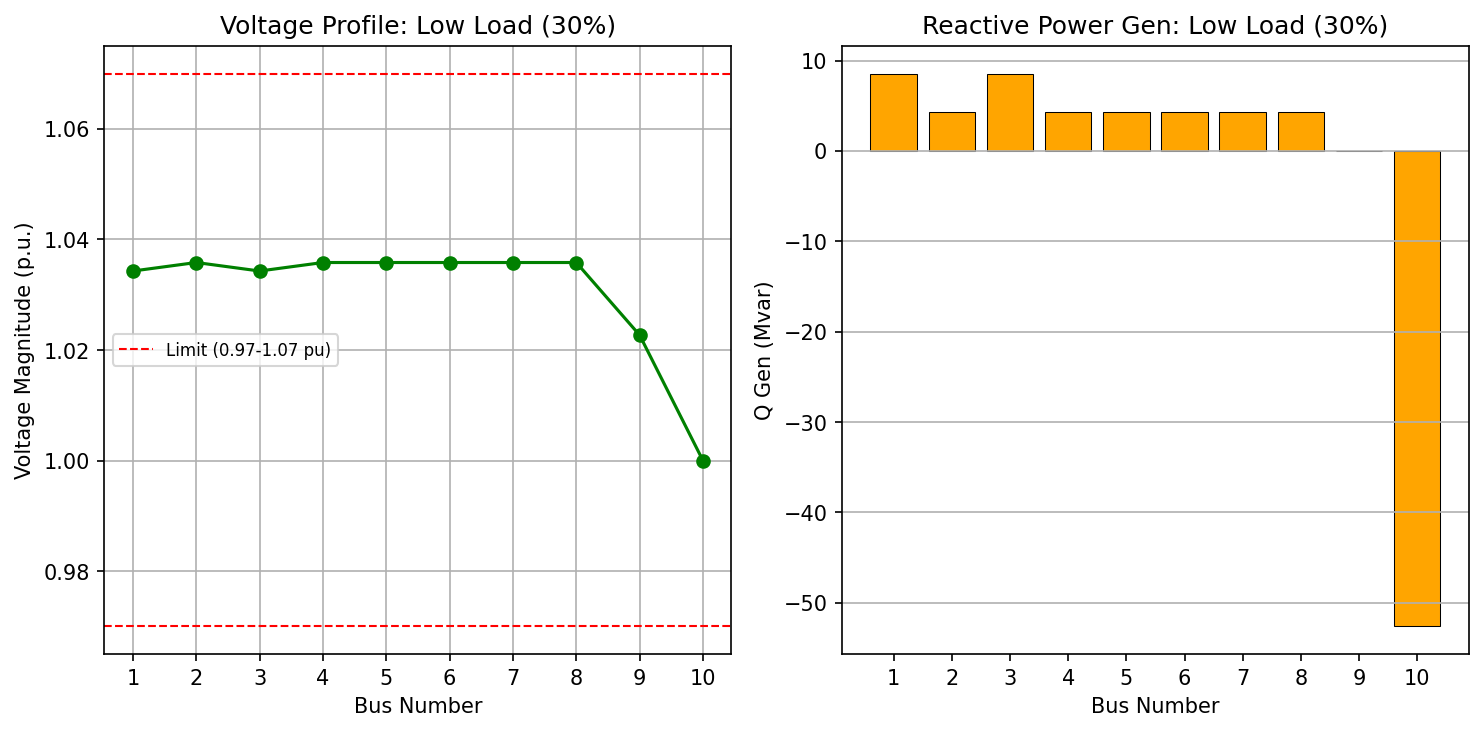
\includegraphics[width=0.7\textwidth]{pf_figs/res_pf_099_low.png}
\caption{Constant PF (0.99) 轻载工况剖面}
\end{figure}

\subsubsection{重载工况 潮流详表}
\begin{longtable}{cccccc}
\caption{Constant PF (0.99) -- 重载工况} \\
\toprule
节点 & 类型 & Vm (pu) & Va (deg) & P Gen (MW) & Q Gen (Mvar) \\
\midrule
\endhead
1 & 1 & 1.0519 & 21.34 & 220.0 & 31.3 \\
2 & 1 & 1.0526 & 21.30 & 110.0 & 15.7 \\
3 & 1 & 1.0519 & 21.34 & 220.0 & 31.3 \\
4 & 1 & 1.0526 & 21.30 & 110.0 & 15.7 \\
5 & 1 & 1.0526 & 21.30 & 110.0 & 15.7 \\
6 & 1 & 1.0526 & 21.30 & 110.0 & 15.7 \\
7 & 1 & 1.0526 & 21.30 & 110.0 & 15.7 \\
8 & 1 & 1.0526 & 21.30 & 110.0 & 15.7 \\
9 & 1 & 1.0426 & 9.22 & 0.0 & 0.0 \\
10 & 3 & 1.0000 & 0.00 & $-$1035.0 & 185.5 \\
\bottomrule
\end{longtable}

\begin{figure}[H]
\centering
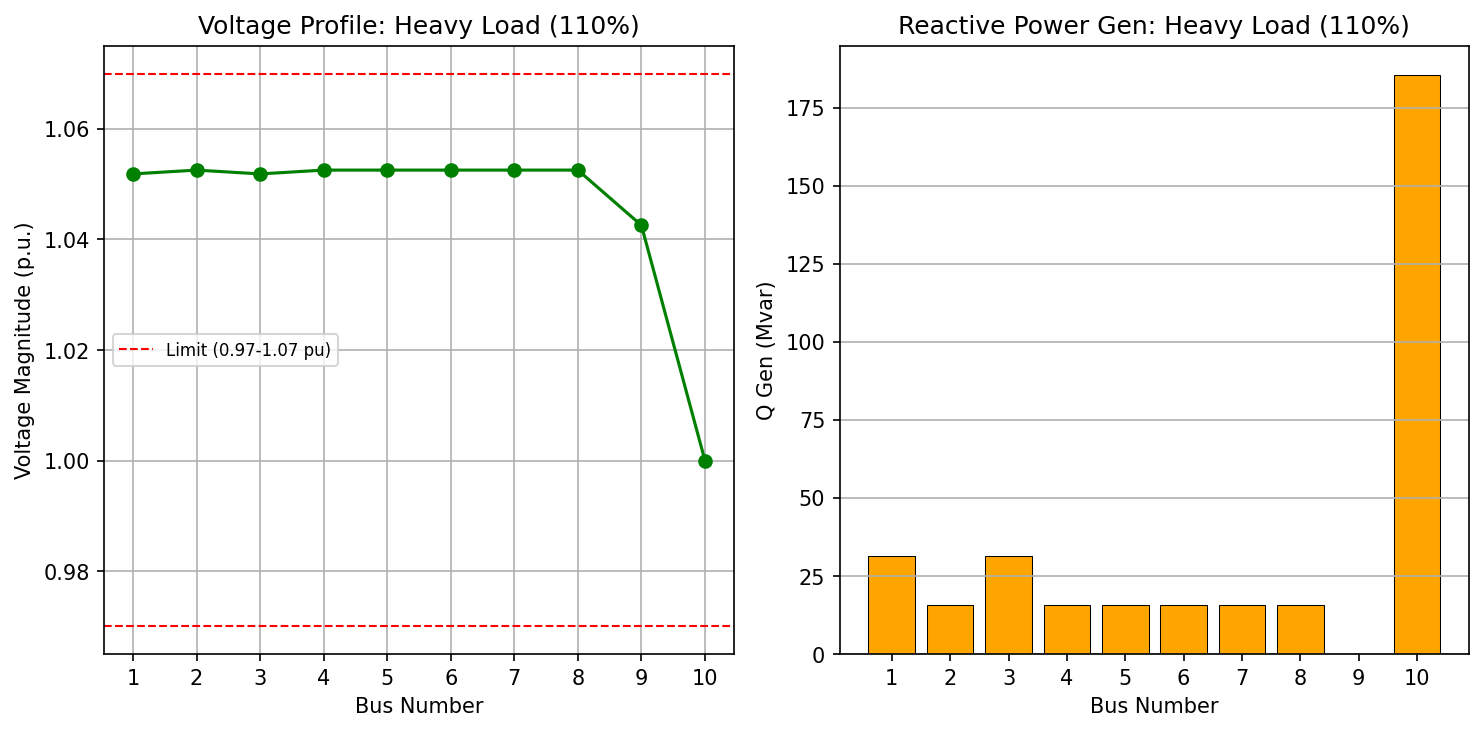
\includegraphics[width=0.7\textwidth]{pf_figs/res_pf_099_heavy.png}
\caption{Constant PF (0.99) 重载工况剖面}
\end{figure}

\subsubsection{故障工况 潮流详表}
\begin{longtable}{cccccc}
\caption{Constant PF (0.99) -- 故障工况} \\
\toprule
节点 & 类型 & Vm (pu) & Va (deg) & P Gen (MW) & Q Gen (Mvar) \\
\midrule
\endhead
1 & 4 & 1.0000 & 0.00 & 0.0 & 0.0 \\
2 & 1 & 1.0469 & 18.14 & 100.0 & 14.2 \\
3 & 1 & 1.0462 & 18.18 & 200.0 & 28.5 \\
4 & 1 & 1.0469 & 18.14 & 100.0 & 14.2 \\
5 & 1 & 1.0469 & 18.14 & 100.0 & 14.2 \\
6 & 1 & 1.0469 & 18.14 & 100.0 & 14.2 \\
7 & 1 & 1.0469 & 18.14 & 100.0 & 14.2 \\
8 & 1 & 1.0469 & 18.14 & 100.0 & 14.2 \\
9 & 1 & 1.0362 & 6.68 & 0.0 & 0.0 \\
10 & 3 & 1.0000 & 0.00 & $-$762.3 & 22.1 \\
\bottomrule
\end{longtable}

\begin{figure}[H]
\centering
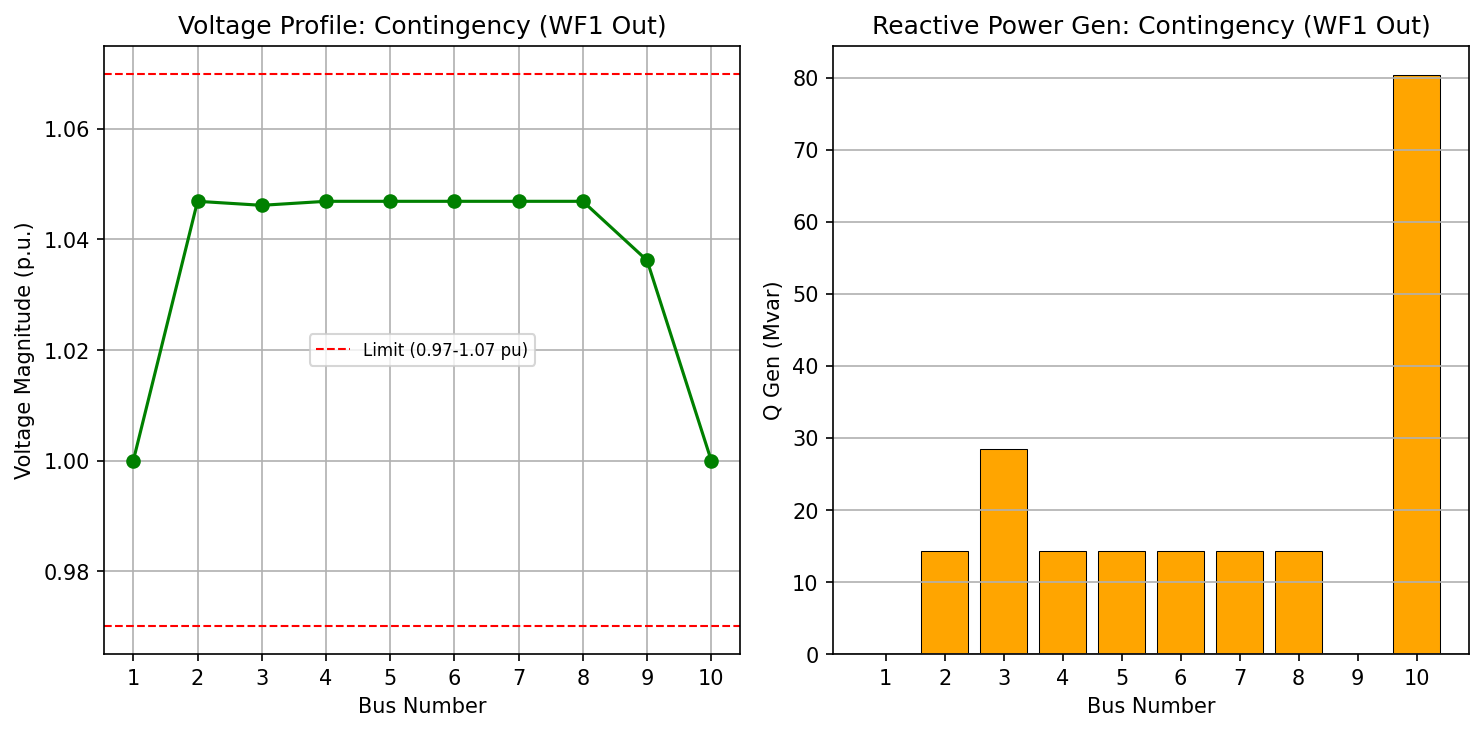
\includegraphics[width=0.7\textwidth]{pf_figs/res_pf_099_trip.png}
\caption{Constant PF (0.99) 故障工况剖面}
\end{figure}

%% ========================= Comparison =============================
\section{三种控制方式综合性能对比}
\begin{figure}[H]
\centering

\includegraphics[width=0.85\textwidth]{pf_figs/final_comp_pv.png}
\caption{控制模式对比与电压稳定性分析 (CloudPSS 线路参数)}
\end{figure}

\textbf{工程结论}:
\begin{enumerate}
    \item \textbf{PF=0.99 的有效性}: 将功率因数目标值从 0.98 调节至 0.99 后，风电场端电压过越现象得到显著抑制。原本在 PF=0.98 下约 1.075 pu 的电压已降至 1.053 pu 左右，完全符合安全范围。
    \item \textbf{电压稳定性平衡}: 虽然 PF=0.99 的无功支撑力度略弱于 PF=0.98，但在 CloudPSS 低阻抗参数下，其 P-V 曲线 collapse 点依然远高于 Q=0 模式，既保证了稳定性，又兼顾了电压上限约束。
    \item \textbf{调节对比}: 
    \begin{itemize}
        \item \textbf{Q=0}: 电压裕度最大，但稳定性最弱。
        \item \textbf{PF=0.98}: 稳定性最强，但在低阻抗系统下易造成电压过快上升。
        \item \textbf{PF=0.99}: 是针对该特定参数系统的“甜点区”(Sweet Spot)，能良好平衡电压上限与稳定性。
    \end{itemize}
    \item \textbf{建议}: 对于 CloudPSS 定义的低阻抗系统，推荐使用 PF=[0.985, 0.995] 范围内的定功率因数控制。
\end{enumerate}

\end{document}
